% ---------------------------------------------------------------------------
%  GPAP -- project status deck, told as the paper we are about to write.
%  Visual-first: every architectural idea is a TikZ figure; text is captions.
%  Compile:  pdflatex gpap_overview.tex   (twice, for the TOC/nav)
%  Deps: base beamer + booktabs + tikz (positioning, arrows.meta). Nothing exotic.
% ---------------------------------------------------------------------------
\documentclass[aspectratio=169,11pt]{beamer}

\usetheme{Boadilla}
\usecolortheme{whale}
\setbeamertemplate{navigation symbols}{}
\setbeamerfont{frametitle}{size=\large}
\setbeamertemplate{itemize items}[circle]

\usepackage[T1]{fontenc}
\usepackage[utf8]{inputenc}
\usepackage{amsmath,amssymb}
\usepackage{booktabs}
\usepackage{xcolor}
\usepackage{tikz}
\usetikzlibrary{positioning,arrows.meta}

\definecolor{gpapblue}{RGB}{31,78,121}
\definecolor{gpapred}{RGB}{170,40,40}
\definecolor{gpapgreen}{RGB}{20,110,70}
\definecolor{gpapgray}{RGB}{115,115,115}
\definecolor{gpapamber}{RGB}{180,120,20}

\newcommand{\good}[1]{\textcolor{gpapgreen}{#1}}
\newcommand{\bad}[1]{\textcolor{gpapred}{#1}}
\newcommand{\rem}[1]{{\footnotesize\textcolor{gpapgray}{#1}}}
\newcommand{\NC}{\textsc{NobleCount}}
\newcommand{\GPAP}{\textsc{Gpap}}
\newcommand{\keyw}[1]{\textcolor{gpapblue}{\textbf{#1}}}

\tikzset{
  bx/.style  = {draw, rounded corners, align=center, minimum height=0.85cm, fill=gpapblue!8,  font=\small},
  bxg/.style = {draw, rounded corners, align=center, minimum height=0.85cm, fill=gpapgreen!12, font=\small},
  bxr/.style = {draw, rounded corners, align=center, minimum height=0.85cm, fill=gpapred!10,  font=\small},
  bxn/.style = {draw, rounded corners, align=center, minimum height=0.85cm, fill=black!4,     font=\small},
  ar/.style  = {-{Latex[length=2mm]}, thick, gpapgray},
}

\title[GPAP]{\GPAP{} --- \textbf{G}PU-\textbf{P}arallel \textbf{A}ssumption \textbf{P}ropagation}
\subtitle{A $K$-parallel BCP engine --- and guaranteed-valid SAT solution sampling built on it}
\author[Y. Shalmon]{Yogev Shalmon}
\institute[Technion]{Technion --- Faculty of Data and Decision Sciences}
\date[\today]{Project status --- \today}

\begin{document}

% == 1 =================================================================
\begin{frame}[plain]
  \titlepage
\end{frame}

% == 2 =================================================================
\begin{frame}{The headline: a BCP engine that runs $300\times$ a CPU core}
  \begin{center}
  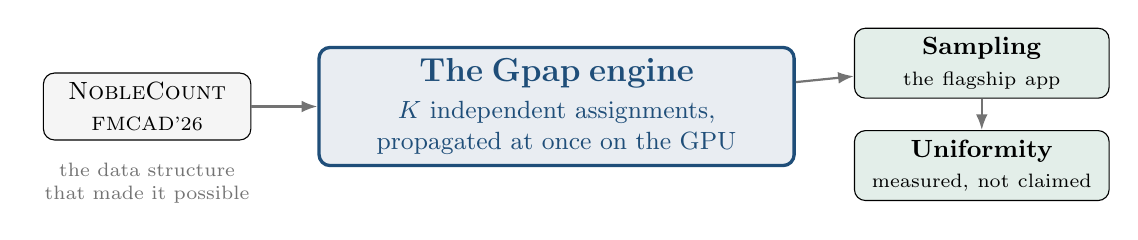
\begin{tikzpicture}[font=\small]
    \node[bxn,text width=2.4cm] (nc) at (0,0) {\NC\\ \scriptsize FMCAD'26};
    \node[draw,very thick,gpapblue,rounded corners,fill=gpapblue!10,
          text width=5.8cm,align=center,minimum height=1.5cm] (eng) at (5.2,0)
      {\large\textbf{The \GPAP{} engine}\\[0.2em]
       \small $K$ independent assignments,\\ propagated at once on the GPU};
    \node[bxg,text width=3.0cm] (s) at (10.6,0.55) {\textbf{Sampling}\\ \scriptsize the flagship app};
    \node[bxg,text width=3.0cm] (u) at (10.6,-0.75) {\textbf{Uniformity}\\ \scriptsize measured, not claimed};
    \draw[ar] (nc) -- (eng);
    \draw[ar] (eng) -- (s);
    \draw[ar] (s) -- (u);
    \node[font=\scriptsize,gpapgray,align=center,text width=2.8cm,anchor=north] at (0,-0.6)
      {the data structure\\ that made it possible};
  \end{tikzpicture}
  \end{center}
  \vspace{0.5em}
  \begin{block}{The result}
    \centering
    \good{\Large $\mathbf{\sim 10^{9}}$ \textbf{propagations/s}} \quad vs.\
    ${\sim}5{\times}10^{6}$ on a single CPU core
    \\[0.3em]
    \good{\textbf{$197$--$631\times$}} --- and \keyw{essentially flat across every benchmark family}
  \end{block}
  \vspace{0.3em}
  \centering
  \keyw{\textbf{But an engine alone is not a contribution.}} So we built the application that needs
  exactly this shape of parallelism --- \good{\textbf{SAT solution sampling}} --- and measured it
  against the state of the art.
\end{frame}

% == 3 =================================================================
\begin{frame}{Where this starts: \NC{} (FMCAD'26)}
  \begin{columns}[T]
    \begin{column}{0.53\textwidth}
      \centering
      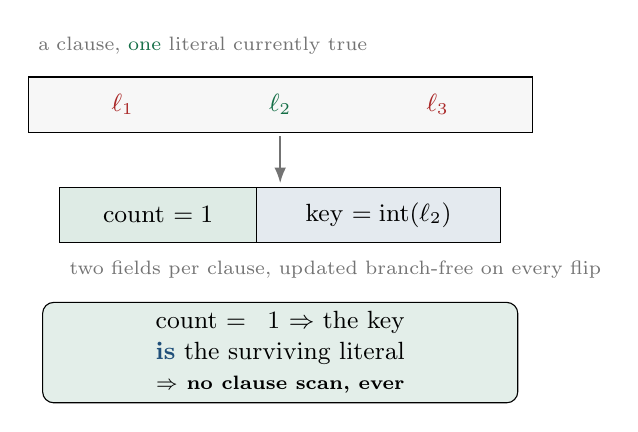
\begin{tikzpicture}[font=\small]
        \draw[fill=black!3] (0,2.2) rectangle (6.4,2.9);
        \node[gpapred]   at (1.2,2.55) {$\ell_1$};
        \node[gpapgreen] at (3.2,2.55) {$\ell_2$};
        \node[gpapred]   at (5.2,2.55) {$\ell_3$};
        \node[font=\scriptsize,gpapgray,anchor=west] at (0,3.3)
          {a clause, \good{one} literal currently true};

        \draw[ar] (3.2,2.15) -- (3.2,1.55);

        \draw[fill=gpapgreen!14] (0.4,0.8) rectangle (2.9,1.5);
        \draw[fill=gpapblue!12]  (2.9,0.8) rectangle (6.0,1.5);
        \node at (1.65,1.15) {count $=1$};
        \node at (4.45,1.15) {key $=\mathrm{int}(\ell_2)$};
        \node[font=\scriptsize,gpapgray,anchor=west] at (0.4,0.45)
          {two fields per clause, updated branch-free on every flip};

        \node[bxg,text width=5.8cm,font=\small] at (3.2,-0.6)
          {count $=1$ $\Rightarrow$ the key \keyw{is} the surviving literal\\
           \scriptsize $\Rightarrow$ \textbf{no clause scan, ever}};
      \end{tikzpicture}
    \end{column}
    \begin{column}{0.44\textwidth}
      \small
      Dropped into ProbCCAnr, the SOTA local-search solver.
      \keyw{No heuristic changes, no re-tuning.}
      \\[0.6em]
      New state of the art on \textbf{FCC} (PAR2 $\bad{-24.8\%}$) \emph{and} \textbf{SC22}.
      \\[0.2em]
      \rem{A data-structure win, orthogonal to heuristic design.}
      \\[0.8em]
      \begin{block}{\small Its own closing sentence}
        \footnotesize
        ``\ldots{} making it \keyw{a promising candidate for parallel clause-state maintenance in
        SIMD- or GPU-based implementations}.''
      \end{block}
    \end{column}
  \end{columns}
\end{frame}

% == 4 =================================================================
\begin{frame}{Same idea, different question}
  \begin{center}
  \resizebox{\textwidth}{!}{%
  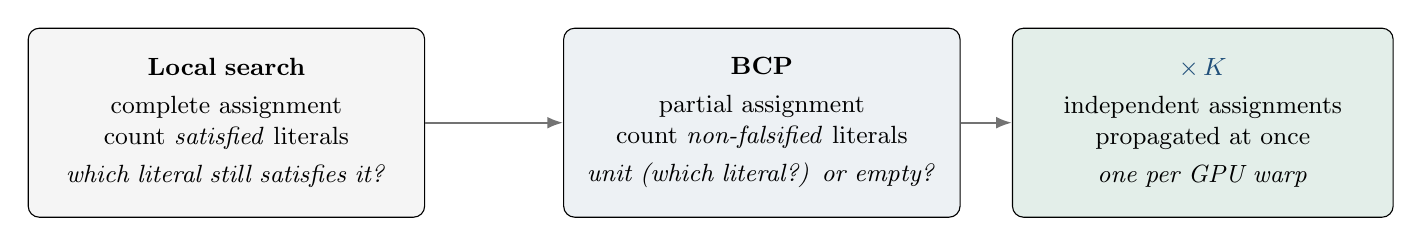
\begin{tikzpicture}[font=\small]
    \node[bxn,text width=4.8cm,minimum height=2.4cm] (l) at (0,0)
      {\textbf{Local search}\\[0.3em]
       complete assignment\\ count \emph{satisfied} literals\\[0.3em]
       \emph{which literal still satisfies it?}};
    \node[bx,text width=4.8cm,minimum height=2.4cm] (r) at (6.8,0)
      {\textbf{BCP}\\[0.3em]
       partial assignment\\ count \emph{non-falsified} literals\\[0.3em]
       \emph{unit (which literal?) or empty?}};
    \draw[ar] (l)--(r);
    \node[bxg,text width=4.6cm,minimum height=2.4cm] (k) at (12.4,0)
      {\keyw{$\times\,K$}\\[0.3em] independent assignments\\ propagated at once\\[0.3em]
       \emph{one per GPU warp}};
    \draw[ar] (r)--(k);
  \end{tikzpicture}}
  \end{center}
  \vspace{0.8em}
  \begin{block}{The primitive, in one line}
    \keyw{Negated occurrence lists}: setting $\ell$ true falsifies $\lnot\ell$ in \emph{exactly}
    the clauses of $\mathrm{occ}[\ell]$ --- a decision touches only what it can affect.
  \end{block}
\end{frame}

% == 5 =================================================================
\begin{frame}{One word per clause --- and the update is its own detector}
  \begin{center}
  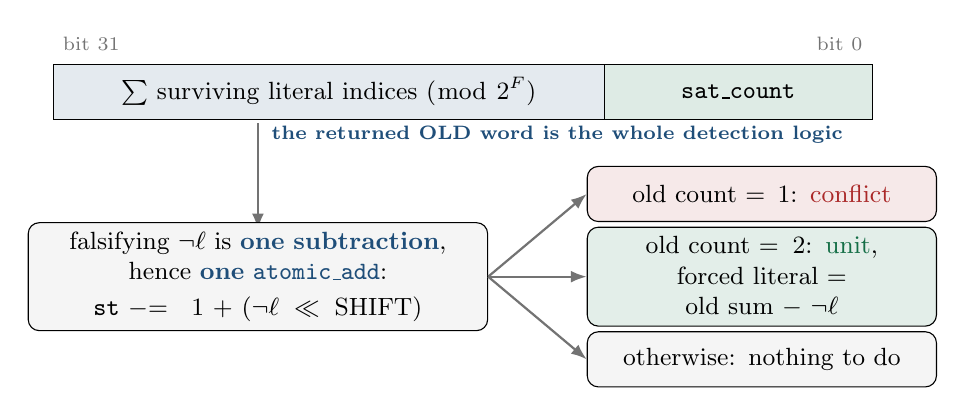
\begin{tikzpicture}[font=\small]
    % --- packed word
    \draw[fill=gpapblue!12]  (0,1.9)  rectangle (7.0,2.6);
    \draw[fill=gpapgreen!14] (7.0,1.9) rectangle (10.4,2.6);
    \node at (3.5,2.25) {$\sum$ surviving literal indices $(\bmod\ 2^{F})$};
    \node at (8.7,2.25) {\texttt{sat\_count}};
    \node[font=\scriptsize,gpapgray,anchor=south west] at (0,2.65) {bit 31};
    \node[font=\scriptsize,gpapgray,anchor=south east] at (10.4,2.65) {bit 0};

    % --- the update
    \draw[ar] (2.6,1.85) -- (2.6,0.5);
    \node[bxn,text width=5.6cm,font=\small,minimum height=1.0cm] (upd) at (2.6,-0.10)
      {falsifying $\lnot\ell$ is \keyw{one subtraction},\\ hence \keyw{one \texttt{atomic\_add}}:\\[0.2em]
       \texttt{st} $\mathrel{-}=\ 1 + (\lnot\ell \ll \mathrm{SHIFT})$};

    % --- the fan
    \node[bxr,text width=4.2cm,minimum height=0.7cm] (o1) at (9.0,0.95)  {old count $=1$: \bad{conflict}};
    \node[bxg,text width=4.2cm,minimum height=0.95cm] (o2) at (9.0,-0.10)
      {old count $=2$: \good{unit},\\ forced literal $=$ old sum $-\ \lnot\ell$};
    \node[bxn,text width=4.2cm,minimum height=0.7cm] (o3) at (9.0,-1.15) {otherwise: nothing to do};
    \draw[ar] (upd.east) -- (o1.west);
    \draw[ar] (upd.east) -- (o2.west);
    \draw[ar] (upd.east) -- (o3.west);
    \node[font=\scriptsize,gpapblue,anchor=south,fill=white,inner sep=1pt] at (6.4,1.55)
      {\textbf{the returned OLD word is the whole detection logic}};
  \end{tikzpicture}
  \end{center}
  \vspace{0.4em}
  \centering
  \rem{The \keyw{assignment} is the same trick: a bitmap where $\ell$ and $\lnot\ell$ share a word,
  so one \texttt{atomic\_or} returns duplicate \emph{and} contradiction together.
  \\ On a CPU, XOR and sum are equivalent --- \NC{} used XOR. On a GPU they are not: the sum makes
  the update an atomic whose \emph{return value} resolves every race --- no locks, no
  \texttt{shfl}/\texttt{ballot}.}
\end{frame}

% == 6 =================================================================
\begin{frame}{A one-slide GPU primer: SMs, warps, and why occupancy is everything}
  \begin{columns}[T]
    \begin{column}{0.46\textwidth}
      \centering
      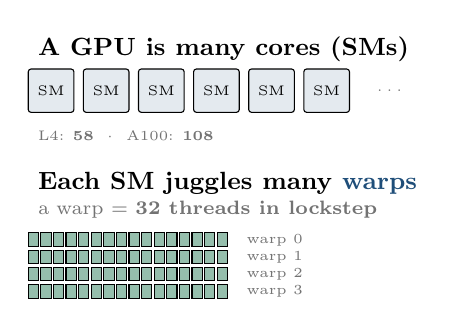
\begin{tikzpicture}[font=\scriptsize]
        \node[font=\small,anchor=west] at (0,3.05) {\textbf{A GPU is many cores (SMs)}};
        \foreach \i in {0,...,5} {
          \draw[fill=gpapblue!12,rounded corners=1pt] (\i*0.7,2.25) rectangle (\i*0.7+0.58,2.8);
          \node[font=\tiny] at (\i*0.7+0.29,2.53) {SM};
        }
        \node[font=\tiny,gpapgray,anchor=west] at (4.3,2.53) {$\dots$};
        \node[font=\tiny,gpapgray,anchor=west] at (0,1.95) {L4: \textbf{58} \ $\cdot$ \ A100: \textbf{108}};

        \node[font=\small,anchor=west] at (0,1.35) {\textbf{Each SM juggles many \keyw{warps}}};
        \node[font=\scriptsize,gpapgray,anchor=west] at (0,1.02) {a warp $=$ \textbf{32 threads in lockstep}};
        \foreach \j in {0,...,3} {
          \foreach \i in {0,...,15} {
            \draw[fill=gpapgreen!45] (\i*0.16,0.55-\j*0.22) rectangle (\i*0.16+0.13,0.72-\j*0.22);
          }
          \node[font=\tiny,gpapgray,anchor=west] at (2.65,0.63-\j*0.22) {warp \j};
        }
      \end{tikzpicture}
    \end{column}
    \begin{column}{0.5\textwidth}
      \small
      \textbf{Memory is ${\sim}400$ cycles away.} A GPU does not hide that with caches --- it hides
      it by having \keyw{another warp ready to run} the moment one stalls.
      \\[0.7em]
      $\Rightarrow$ \good{\textbf{You must supply enough independent work.}}
      \\[0.3em]
      Too few warps and the machine sits idle waiting on DRAM, no matter how fast the arithmetic
      is.
      \\[0.7em]
      \rem{``Occupancy'' $=$ resident warps $/$ the maximum the SMs can hold.}
    \end{column}
  \end{columns}
  \vspace{0.5em}
  \centering
  \rem{This is the whole design constraint for what follows: \keyw{our unit of parallelism is one
  assignment} --- so the question is always \emph{how many can we keep in flight?}}
\end{frame}

% == 7 =================================================================
\begin{frame}{The architecture: one assignment per warp}
  \begin{columns}[T]
    % ============ LEFT: small formula, K huge ============
    \begin{column}{0.48\textwidth}
      \centering
      \textbf{\color{gpapblue}Small formula} $\Rightarrow$ $K$ \textbf{huge} (${\sim}100$k rows)
      \\[0.4em]
      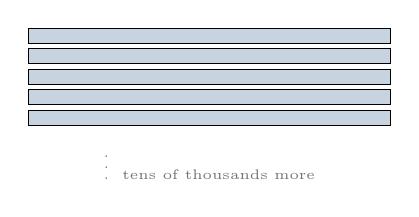
\begin{tikzpicture}[font=\tiny]
        \foreach \y in {0,1,2,3,4} { \draw[fill=gpapblue!25] (0,\y*0.26) rectangle (4.6,\y*0.26+0.19); }
        \node[gpapgray,anchor=north] at (2.3,-0.05) {$\vdots$ \ tens of thousands more};
      \end{tikzpicture}
      \\[0.5em]
      \small
      \good{\textbf{GPU oversubscribed}} --- a stall is hidden by the next row.
      \bad{More compute per row buys nothing}: we are \keyw{waiting on memory}.
      \\[0.5em]
      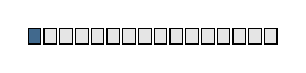
\begin{tikzpicture}
        \foreach \i in {0,...,15} { \draw[fill=black!10] (\i*0.2,0) rectangle (\i*0.2+0.16,0.2); }
        \draw[fill=gpapblue!85] (0,0) rectangle (0.16,0.2);
      \end{tikzpicture}
      \\[0.2em]
      \textbf{SCALAR}: \keyw{1 lane of 32} walks $\mathrm{occ}[\ell]$ --- \good{no atomics needed}
    \end{column}
    % ============ RIGHT: big formula, K tiny ============
    \begin{column}{0.48\textwidth}
      \centering
      \textbf{\color{gpapgreen}Big formula} $\Rightarrow$ VRAM caps $K$ \textbf{low} (hundreds)
      \\[0.4em]
      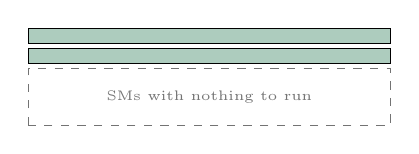
\begin{tikzpicture}[font=\tiny]
        \foreach \y in {3,4} { \draw[fill=gpapgreen!35] (0,\y*0.26) rectangle (4.6,\y*0.26+0.19); }
        \draw[dashed,gpapgray] (0,0) rectangle (4.6,0.72);
        \node[gpapgray] at (2.3,0.36) {SMs with nothing to run};
      \end{tikzpicture}
      \\[0.5em]
      \small
      \bad{\textbf{GPU starved}} --- too few rows to hide latency, most of the machine idles.
      \good{\textbf{Now we \emph{want} more work per row.}}
      \\[0.5em]
      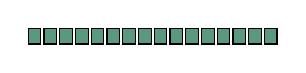
\begin{tikzpicture}
        \foreach \i in {0,...,15} { \draw[fill=gpapgreen!70] (\i*0.2,0) rectangle (\i*0.2+0.16,0.2); }
      \end{tikzpicture}
      \\[0.2em]
      \textbf{WAVE}: \keyw{all 32 lanes} update clauses \emph{inside one assignment}
    \end{column}
  \end{columns}
  \vspace{0.5em}
  \centering
  \keyw{One dispatch rule, measured}: WAVE while $K < 30\times$ resident warps, SCALAR beyond.
  \\[0.2em]
  \rem{Same state, bit-identical results --- the formula size that starves one variant is exactly
  what feeds the other.}
\end{frame}

% == 8 =================================================================
\begin{frame}{The tool}
  \begin{center}
  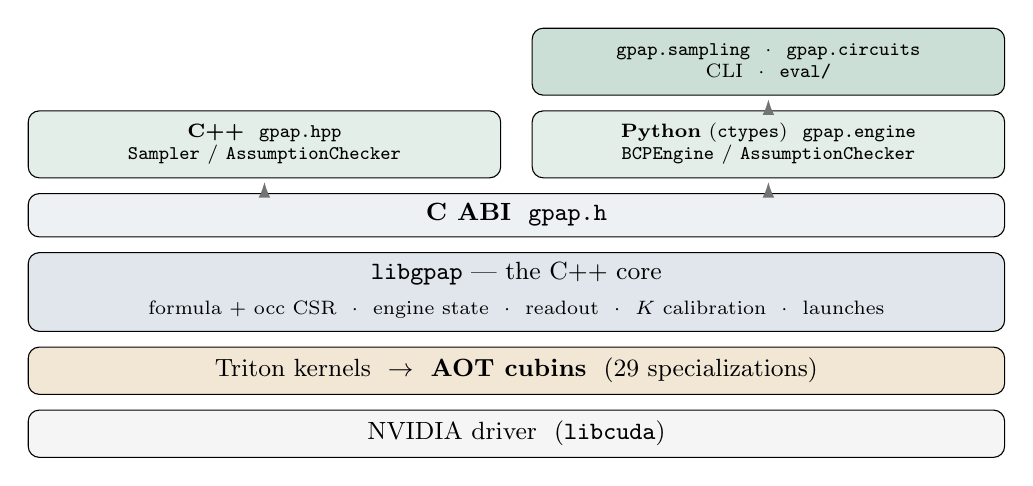
\begin{tikzpicture}[font=\small]
    \draw[fill=black!4,rounded corners]      (0,0)    rectangle (12.4,0.6);
    \node at (6.2,0.3) {NVIDIA driver \ (\texttt{libcuda})};

    \draw[fill=gpapamber!18,rounded corners] (0,0.8)  rectangle (12.4,1.4);
    \node at (6.2,1.1) {Triton kernels \ $\rightarrow$ \ \textbf{AOT cubins} \ (29 specializations)};

    \draw[fill=gpapblue!14,rounded corners]  (0,1.6)  rectangle (12.4,2.6);
    \node[font=\small] at (6.2,2.33) {\textbf{\texttt{libgpap}} --- the C++ core};
    \node[font=\scriptsize] at (6.2,1.88)
      {formula $+$ occ CSR \ $\cdot$ \ engine state \ $\cdot$ \ readout \ $\cdot$ \ $K$ calibration \ $\cdot$ \ launches};

    \draw[fill=gpapblue!8,rounded corners]   (0,2.8)  rectangle (12.4,3.35);
    \node[font=\small] at (6.2,3.08) {\textbf{C ABI} \ \texttt{gpap.h}};

    \draw[fill=gpapgreen!12,rounded corners] (0,3.55)   rectangle (6.0,4.4);
    \node[font=\scriptsize,align=center] at (3.0,3.98)
      {\textbf{C++} \ \texttt{gpap.hpp}\\ \texttt{Sampler} / \texttt{AssumptionChecker}};
    \draw[fill=gpapgreen!12,rounded corners] (6.4,3.55) rectangle (12.4,4.4);
    \node[font=\scriptsize,align=center] at (9.4,3.98)
      {\textbf{Python} (\texttt{ctypes}) \ \texttt{gpap.engine}\\ \texttt{BCPEngine} / \texttt{AssumptionChecker}};

    \draw[fill=gpapgreen!22,rounded corners] (6.4,4.6)  rectangle (12.4,5.45);
    \node[font=\scriptsize,align=center] at (9.4,5.03)
      {\texttt{gpap.sampling} \ $\cdot$ \ \texttt{gpap.circuits}\\ CLI \ $\cdot$ \ \texttt{eval/}};

    \draw[ar] (3.0,3.4) -- (3.0,3.5);
    \draw[ar] (9.4,3.4) -- (9.4,3.5);
    \draw[ar] (9.4,4.45) -- (9.4,4.55);
  \end{tikzpicture}
  \end{center}
  \vspace{0.4em}
  \centering
  \rem{\keyw{One implementation}: both faces link the same library, so there is no second engine to
  drift. The build needs no CUDA toolkit and no \texttt{nvcc}; the runtime needs \texttt{libcuda}
  alone.}
\end{frame}

% == 9 =================================================================
\begin{frame}{What is a $K$-parallel BCP primitive good for?}
  \begin{center}
  \resizebox{\textwidth}{!}{%
  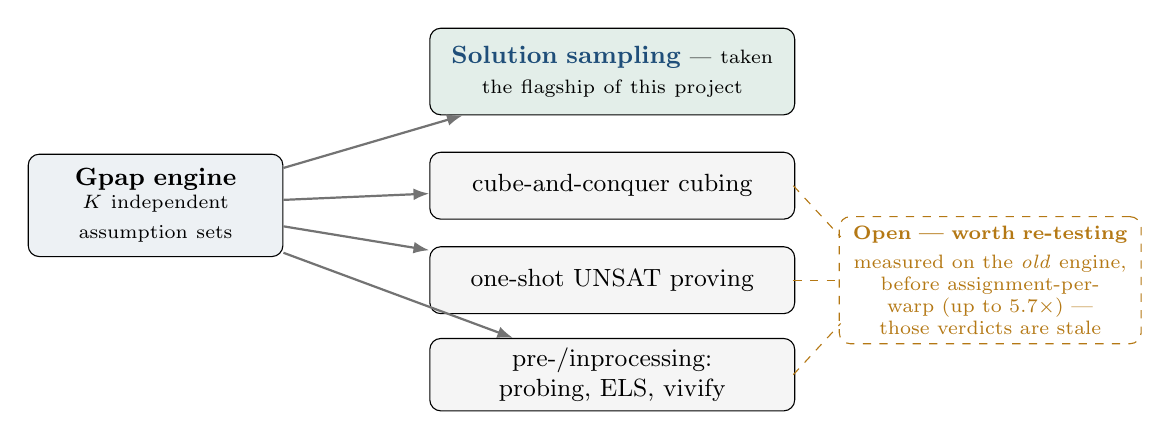
\begin{tikzpicture}[font=\small]
    \node[bx,text width=3.0cm,minimum height=1.3cm] (e) at (0,0)
      {\textbf{\GPAP{} engine}\\ \scriptsize $K$ independent\\ \scriptsize assumption sets};

    \node[bxg,text width=4.4cm,minimum height=1.1cm] (s) at (5.8,1.7)
      {\keyw{Solution sampling} \scriptsize --- taken\\ \scriptsize the flagship of this project};
    \node[bxn,text width=4.4cm] (c) at (5.8,0.25) {cube-and-conquer cubing};
    \node[bxn,text width=4.4cm] (u) at (5.8,-0.95) {one-shot UNSAT proving};
    \node[bxn,text width=4.4cm] (p) at (5.8,-2.15) {pre-/inprocessing: probing, ELS, vivify};

    \draw[ar] (e) -- (s); \draw[ar] (e) -- (c); \draw[ar] (e) -- (u); \draw[ar] (e) -- (p);

    \node[draw,dashed,rounded corners,gpapamber,text width=3.6cm,align=center,font=\scriptsize]
      at (10.6,-0.95)
      {\textcolor{gpapamber}{\textbf{Open --- worth re-testing}}\\[0.3em]
       measured on the \emph{old} engine, before assignment-per-warp (up to $5.7\times$)
       --- those verdicts are stale};
    \draw[gpapamber,dashed] (8.1,0.25) -- (8.7,-0.4);
    \draw[gpapamber,dashed] (8.1,-0.95) -- (8.7,-0.95);
    \draw[gpapamber,dashed] (8.1,-2.15) -- (8.7,-1.5);
  \end{tikzpicture}}
  \end{center}
  \centering
  \rem{Sampling fits the layout exactly: millions of independent randomized completions over one
  shared, read-only occurrence structure.}
\end{frame}

% == 10 ================================================================
\begin{frame}{The sampler: inspired by CMSGen, run $K$ at a time}
  \begin{center}
  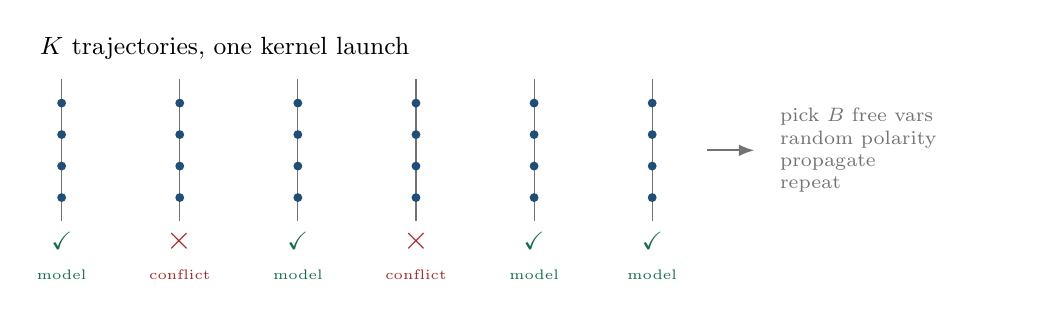
\begin{tikzpicture}[font=\scriptsize]
    \node[font=\small,anchor=west] at (-0.4,2.4) {$K$ trajectories, one kernel launch};
    \foreach \x in {0, 1.5, 3.0, 4.5, 6.0, 7.5} {
      \draw[gpapgray] (\x,2.0) -- (\x,0.2);
      \foreach \y in {1.7,1.3,0.9,0.5} { \fill[gpapblue] (\x,\y) circle (1.6pt); }
    }
    \foreach \x in {1.5, 4.5} {
      \node[gpapred,font=\large] at (\x,-0.05) {$\times$};
      \node[gpapred,font=\tiny,anchor=north] at (\x,-0.3) {conflict};
    }
    \foreach \x in {0, 3.0, 6.0, 7.5} {
      \node[gpapgreen,font=\small] at (\x,-0.05) {$\checkmark$};
      \node[gpapgreen,font=\tiny,anchor=north] at (\x,-0.3) {model};
    }
    \draw[ar] (8.2,1.1) -- (8.8,1.1);
    \node[font=\scriptsize,gpapgray,align=left,text width=3.0cm,anchor=west] at (9.0,1.1)
      {pick $B$ free vars\\ random polarity\\ propagate\\ repeat};
  \end{tikzpicture}
  \end{center}
  \vspace{0.5em}
  \begin{columns}[T]
    \begin{column}{0.46\textwidth}
      \small
      \keyw{Inspired by CMSGen's Algorithm 1} --- random variable, random polarity, propagate ---
      but $K$ trajectories at a time.
      \\[0.3em]
      \rem{The structural difference: CMSGen backtracks out of a conflict; \GPAP{}
      \emph{discards} the trajectory.}
    \end{column}
    \begin{column}{0.5\textwidth}
      \begin{block}{Two consequences}
        \small
        \good{Every emitted row is a real model} --- no gradient, no rounding, no repair.\\[0.3em]
        Discarding \emph{is} rejection sampling $\Rightarrow$ an exactness knob (later).
      \end{block}
    \end{column}
  \end{columns}
\end{frame}

% == 11 ================================================================
\begin{frame}{The flagship pipeline}
  \begin{center}
  \resizebox{\textwidth}{!}{%
  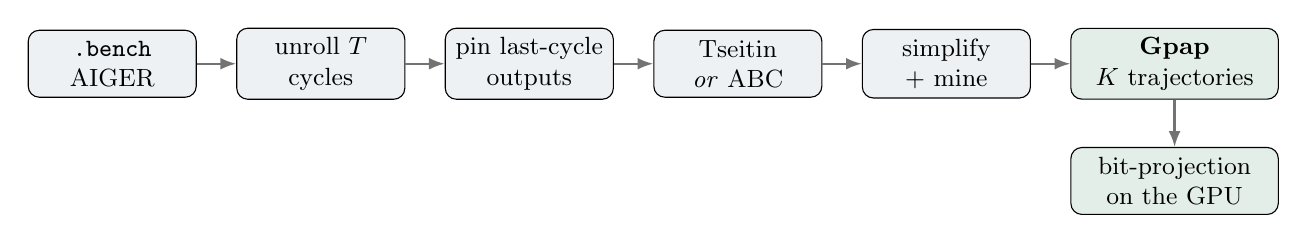
\begin{tikzpicture}[font=\scriptsize, node distance=5mm]
    \node[bx,text width=1.9cm] (a) {\texttt{.bench}\\ AIGER};
    \node[bx,text width=1.9cm,right=of a] (b) {unroll $T$\\ cycles};
    \node[bx,text width=1.9cm,right=of b] (c) {pin last-cycle\\ outputs};
    \node[bx,text width=1.9cm,right=of c] (d) {Tseitin\\ \emph{or} ABC};
    \node[bx,text width=1.9cm,right=of d] (e) {simplify\\ $+$ mine};
    \node[bxg,text width=2.4cm,right=of e] (f) {\textbf{\GPAP{}}\\ $K$ trajectories};
    \node[bxg,text width=2.4cm,below=6mm of f] (g) {bit-projection\\ on the GPU};
    \draw[ar] (a)--(b); \draw[ar] (b)--(c); \draw[ar] (c)--(d);
    \draw[ar] (d)--(e); \draw[ar] (e)--(f); \draw[ar] (f)--(g);
  \end{tikzpicture}}
  \end{center}
  \vspace{0.8em}
  \begin{columns}[T]
    \begin{column}{0.3\textwidth}
      \keyw{Support} $=$ primary inputs $\times$ cycles.
      \rem{Only the bit matrix leaves the device.}
    \end{column}
    \begin{column}{0.32\textwidth}
      \keyw{Encoder} is a choice: native Tseitin, or ABC.
      \rem{Same projected solution set --- gated by set-equality tests.}
    \end{column}
    \begin{column}{0.32\textwidth}
      \keyw{Config} is per instance: a bandit measures at full $K$.
      \rem{The right answer is instance-dependent, so we never guess it.}
    \end{column}
  \end{columns}
\end{frame}

% == 12 ================================================================
\begin{frame}{The question we asked before a reviewer could: why not just simulate?}
  \begin{columns}[T]
    \begin{column}{0.56\textwidth}
      \resizebox{\linewidth}{!}{%
      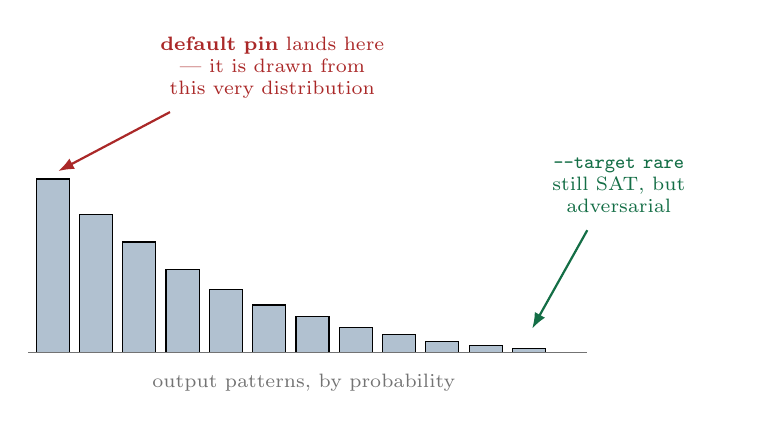
\begin{tikzpicture}[font=\scriptsize]
        \foreach \i/\h in {0/2.2, 1/1.75, 2/1.4, 3/1.05, 4/0.8, 5/0.6, 6/0.45, 7/0.32, 8/0.22, 9/0.14, 10/0.09, 11/0.05} {
          \draw[fill=gpapblue!35] (\i*0.55,0) rectangle (\i*0.55+0.42,\h);
        }
        \draw[gpapgray] (-0.1,0) -- (7.0,0);
        \node[font=\scriptsize,gpapgray,anchor=north] at (3.4,-0.15) {output patterns, by probability};

        \draw[ar,gpapred] (1.7,3.05) -- (0.28,2.3);
        \node[font=\scriptsize,gpapred,align=center,text width=3.4cm,anchor=south] at (3.0,3.1)
          {\textbf{default pin} lands here --- it is drawn from this very distribution};
        \draw[ar,gpapgreen] (7.0,1.55) -- (6.3,0.3);
        \node[font=\scriptsize,gpapgreen,align=center,text width=2.6cm,anchor=south] at (7.4,1.65)
          {\texttt{-{}-target rare}\\ still SAT, but adversarial};
      \end{tikzpicture}}
    \end{column}
    \begin{column}{0.42\textwidth}
      \small
      At default pins, plain CPU simulation $+$ filtering \bad{beat us on 17/19}.
      \\[0.6em]
      \keyw{So we changed the protocol, not the claim}: pin a \emph{rare} output pattern ---
      still reachable, but adversarial for rejection.
      \\[0.6em]
      \good{\textbf{At rare targets it cannot play at all}}: on EPFL, \good{0 hits in ${\sim}10$M
      random patterns} while \GPAP{} samples at $89$--$100\%$ success.
    \end{column}
  \end{columns}
  \vspace{0.5em}
  \centering
  \rem{Rejection is not just a rival --- it picks our targets and audits every emitted sample.}
\end{frame}

% == 13 ================================================================
\begin{frame}{Headline: \GPAP{} vs.\ CMSGen, 357 cells, 0 errors}
  \centering
  \small
  \begin{tabular}{@{}llrrr@{}}
    \toprule
    family & targets & \textbf{Colab L4} & 4080 laptop & wins \\
    \midrule
    ITC'99 $+$ ISCAS-89 seq, $T{=}25$ & \keyw{rare} & \good{$39.1\times$}  & $36.5\times$ & 17/18 \\
    ISCAS-85 combinational            & \keyw{rare} & \good{$615\times$}   & $538\times$  & 10/10 \\
    HWMCC'17, $T{=}25$                & \keyw{rare} & \good{$196\times$}   & $156\times$  & 7/7 \\
    EPFL combinational                & \keyw{rare} & $9.4\times$          & $6.4\times$  & 13/17 \\
    Sketch / \texttt{sk\_} CNFs       & ---         & \good{$98.9\times$}  & $46.2\times$ & 27/29 \\
    \bottomrule
  \end{tabular}
  \\[1.0em]
  \begin{columns}[T]
    \begin{column}{0.48\textwidth}
      \bad{\textbf{Every ratio is higher on the L4 --- and none of that is \GPAP{}.}}
      \\[0.4em]
      \small
      Paired on identical cells: \GPAP{} $0.96\times$, \keyw{CMSGen $0.41\times$}.
      The Colab host is a slower CPU, and CMSGen is single-core.
    \end{column}
    \begin{column}{0.48\textwidth}
      \good{\textbf{The rule we adopted: never quote a ratio without the CPU.}}
      \\[0.4em]
      \small
      Otherwise a reviewer reads $98.9\times$ and correctly calls it a rigged baseline.
    \end{column}
  \end{columns}
  \vspace{0.5em}
  \centering
  \rem{$357$ cells, \good{0 skipped, 0 errors, 0 unsound}. Per instance at its best encoder;
  geomeans exclude tautological pins and instances that need no search. Full tables in the
  appendix.}
\end{frame}

% == 14 ================================================================
\begin{frame}{Is the speedup the engine, or the benchmark?}
  \centering
  \small
  \begin{tabular}{@{}lrrrr@{}}
    \toprule
     & \multicolumn{2}{c}{implications$/$s} & \multicolumn{2}{c}{implications$/$sample} \\
    \cmidrule(lr){2-3}\cmidrule(lr){4-5}
    family (\keyw{rare}) & \GPAP{} & CMSGen & \GPAP{} & CMSGen \\
    \midrule
    ISCAS-85 combinational      & $1.05{\times}10^{9}$ & $1.67{\times}10^{6}$ & $517$      & $507$      \\
    ITC'99/ISCAS-89, $T{=}25$   & $1.14{\times}10^{9}$ & $5.20{\times}10^{6}$ & $30{,}538$ & $5{,}422$  \\
    HWMCC'17, $T{=}25$          & $1.05{\times}10^{9}$ & $4.58{\times}10^{6}$ & $12{,}615$ & $10{,}737$ \\
    EPFL combinational          & $1.08{\times}10^{9}$ & $2.14{\times}10^{6}$ & $12{,}139$ & $226$      \\
    Sketch / \texttt{sk\_} CNFs & $1.00{\times}10^{9}$ & $4.23{\times}10^{6}$ & $851$      & $355$      \\
    \bottomrule
  \end{tabular}
  \\[0.6em]
  \begin{columns}[T]
    \begin{column}{0.44\textwidth}
      \good{\textbf{The engine's rate is flat}} --- ${\sim}10^{9}$/s everywhere, spread only
      $1.41\times$, while the \emph{sample} ratio moves ${\sim}2$ orders.
      \\[0.3em]
      \keyw{It is a property of the GPU, not the benchmark.}
    \end{column}
    \begin{column}{0.54\textwidth}
      \centering
      $\text{samples/s ratio}=\dfrac{\text{impl/s ratio}}{\text{impl/sample ratio}}$
      \\[0.4em]
      \raggedright\small
      Exact on $9/9$ families. The engine buys $197$--$631\times$;
      \bad{rejection spends part back} --- $1.0\times$ on ISCAS-85, $5.6\times$ on sequential,
      \bad{$53.7\times$ on EPFL}.
    \end{column}
  \end{columns}
  \vspace{0.3em}
  \centering
  \rem{We discard a conflicted trajectory; CMSGen backtracks and keeps the partial work. EPFL pays
  the most --- and is the one family with an instance we could not sample at all.}
\end{frame}

% == 15 ================================================================
\begin{frame}{Who else puts SAT sampling on a GPU?}
  \begin{center}
  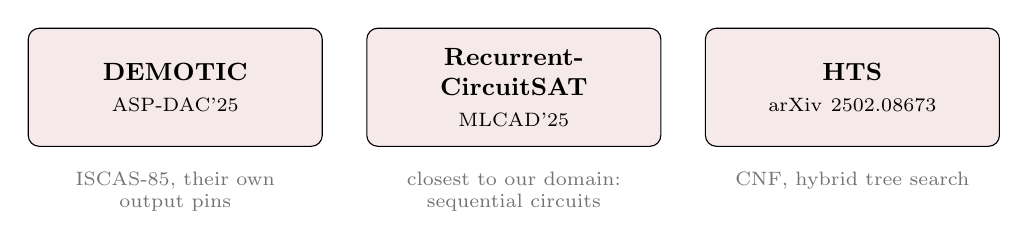
\begin{tikzpicture}[font=\scriptsize]
    \node[bxr,text width=3.5cm,minimum height=1.5cm] (d) at (0,0)
      {\textbf{DEMOTIC}\\ \scriptsize ASP-DAC'25};
    \node[bxr,text width=3.5cm,minimum height=1.5cm] (r) at (4.3,0)
      {\textbf{Recurrent-CircuitSAT}\\ \scriptsize MLCAD'25};
    \node[bxr,text width=3.5cm,minimum height=1.5cm] (h) at (8.6,0)
      {\textbf{HTS}\\ \scriptsize arXiv 2502.08673};
    \node[font=\scriptsize,gpapgray,text width=3.5cm,align=center,anchor=north] at (0,-0.95)
      {ISCAS-85, their own\\ output pins};
    \node[font=\scriptsize,gpapgray,text width=3.5cm,align=center,anchor=north] at (4.3,-0.95)
      {closest to our domain:\\ sequential circuits};
    \node[font=\scriptsize,gpapgray,text width=3.5cm,align=center,anchor=north] at (8.6,-0.95)
      {CNF, hybrid tree search};
  \end{tikzpicture}
  \end{center}
  \vspace{0.4em}
  \begin{columns}[T]
    \begin{column}{0.48\textwidth}
      \bad{\textbf{They all do the same thing}}: relax the circuit to a \emph{continuous}
      function and follow the gradient towards a solution.
      \\[0.4em]
      \small
      Fast, and GPU-native --- but a gradient lands \emph{near} a solution, so the output must be
      rounded and repaired, and \bad{may not satisfy the formula}.
    \end{column}
    \begin{column}{0.48\textwidth}
      \good{\textbf{\GPAP{} is discrete throughout}}: every trajectory is real propagation, so
      \good{every emitted row is a model by construction} --- nothing to verify, nothing to repair.
      \\[0.4em]
      \rem{We compare on \emph{their} metric: unique solutions per second of their own reported
      runtime.}
    \end{column}
  \end{columns}
\end{frame}

% == 16 ================================================================
\begin{frame}{Versus the GPU gradient samplers}
  \centering
  \small
  \begin{tabular}{@{}llrr@{}}
    \toprule
    rival & pins used & GPAP $/$ rival & GPAP wins \\
    \midrule
    DEMOTIC   & \emph{their} ISCAS-85 pins & $2.5\times$        & 19/20 \\
    DEMOTIC   & our \keyw{rare} pins       & $2{,}427\times$    & 16/16 \\
    Recurrent & \emph{their} target table  & $4.4\times$        & 6/6   \\
    Recurrent & our \keyw{rare} pins       & \good{$635\times$} & 5/6   \\
    HTS       & our CNFs                   & $1{,}584\times$    & 13/14 \\
    \bottomrule
  \end{tabular}
  \\[1.0em]
  \begin{columns}[T]
    \begin{column}{0.52\textwidth}
      \keyw{\textbf{The protocol matters more than the rival.}}
      \\[0.4em]
      \small
      Recurrent-CircuitSAT reads \textbf{$4.4\times$} on \emph{their} pins and
      \textbf{$635\times$} on ours --- \bad{a $140$-fold swing}, same sampler, same GPU, same day.
      Only the target changed.
    \end{column}
    \begin{column}{0.44\textwidth}
      \good{\textbf{Their pins are easy by construction}}, so a win there is not a sampling
      result.
      \\[0.4em]
      \bad{Honest losses}: the ``service'' family --- jointly-constrained instances that need
      clause \emph{learning}.
    \end{column}
  \end{columns}
  \vspace{0.4em}
  \centering
  \rem{7 rival runs failed (timeout / no gradient path): reported, never counted as zeros.
  Cells where \emph{we} emitted nothing are counted as losses.}
\end{frame}

% == 17 ================================================================
\begin{frame}{Does that verdict survive a different GPU?}
  \centering
  \small
  \begin{tabular}{@{}llrrc@{}}
    \toprule
    rival & protocol & \multicolumn{2}{c}{GPAP $/$ rival (geomean)} & GPAP wins \\
    \cmidrule(lr){3-4}
     & & 4080 laptop & \textbf{L4} & on L4 \\
    \midrule
    DEMOTIC   & their ISCAS-85 pins     & $2.9\times$     & $2.5\times$     & \good{19/20} \\
    DEMOTIC   & our \keyw{rare} pins    & $7{,}704\times$ & $2{,}427\times$ & \good{16/16} \\
    Recurrent & our \keyw{rare} pins    & $599\times$     & $422\times$     & \good{3/3} \\
    HTS       & our CNFs, both encoders & ---             & $2{,}042\times$ & \good{10/10} \\
    \bottomrule
  \end{tabular}
  \\[1.0em]
  \begin{columns}[T]
    \begin{column}{0.48\textwidth}
      \good{\textbf{What transfers: the verdict.}}
      \\[0.4em]
      \small
      Win counts are \emph{identical} on both cards, instance by instance --- because both sides
      share the GPU.
    \end{column}
    \begin{column}{0.48\textwidth}
      \bad{\textbf{What does not: the magnitude.}}
      \\[0.4em]
      \small
      At rare pins the rival scores ${\approx}0$, so the ratio has a near-zero denominator.
      \keyw{Read these as orders of magnitude, never as constants.}
    \end{column}
  \end{columns}
  \vspace{0.5em}
  \centering
  \rem{\bad{Honest}: \texttt{c1355} loses on both cards; at a rare \texttt{b11} pin \emph{neither}
  sampler finds anything.}
\end{frame}

% == 18 ================================================================
\begin{frame}{What ``uniform'' means --- and why a sampler lives or dies by it}
  \begin{center}
  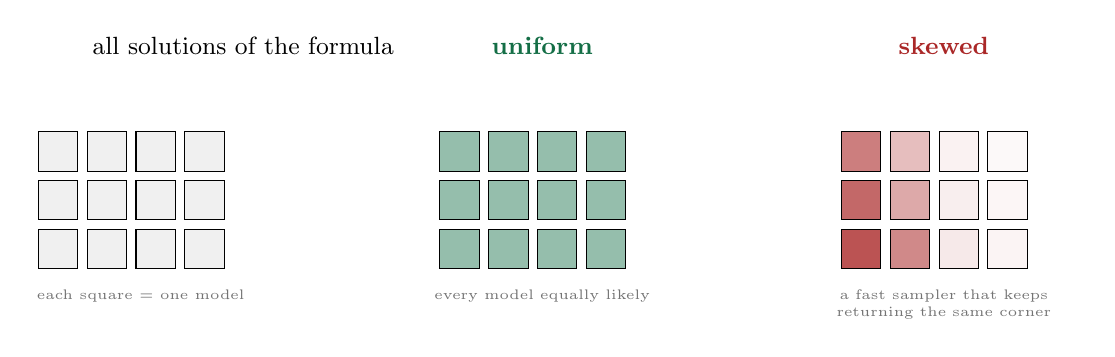
\begin{tikzpicture}[font=\scriptsize]
    % --- the solution space
    \node[font=\small,anchor=south] at (2.6,2.6) {all solutions of the formula};
    \foreach \i/\j in {0/0, 1/0, 2/0, 3/0, 0/1, 1/1, 2/1, 3/1, 0/2, 1/2, 2/2, 3/2} {
      \draw[fill=black!6] (\i*0.62,\j*0.62) rectangle (\i*0.62+0.5,\j*0.62+0.5);
    }
    \node[font=\tiny,gpapgray,anchor=north] at (1.3,-0.15) {each square $=$ one model};

    % --- uniform
    \node[font=\small,gpapgreen,anchor=south] at (6.4,2.6) {\good{\textbf{uniform}}};
    \foreach \i/\j in {0/0, 1/0, 2/0, 3/0, 0/1, 1/1, 2/1, 3/1, 0/2, 1/2, 2/2, 3/2} {
      \draw[fill=gpapgreen!45] (5.1+\i*0.62,\j*0.62) rectangle (5.1+\i*0.62+0.5,\j*0.62+0.5);
    }
    \node[font=\tiny,gpapgray,anchor=north,text width=3.0cm,align=center] at (6.4,-0.15)
      {every model equally likely};

    % --- skewed
    \node[font=\small,gpapred,anchor=south] at (11.5,2.6) {\bad{\textbf{skewed}}};
    \foreach \i/\j/\o in {0/0/80, 1/0/55, 2/0/10, 3/0/5, 0/1/70, 1/1/40, 2/1/8, 3/1/4,
                          0/2/60, 1/2/30, 2/2/6, 3/2/3} {
      \draw[fill=gpapred!\o] (10.2+\i*0.62,\j*0.62) rectangle (10.2+\i*0.62+0.5,\j*0.62+0.5);
    }
    \node[font=\tiny,gpapgray,anchor=north,text width=3.4cm,align=center] at (11.5,-0.15)
      {a fast sampler that keeps\\ returning the same corner};
  \end{tikzpicture}
  \end{center}
  \vspace{0.5em}
  \begin{columns}[T]
    \begin{column}{0.5\textwidth}
      \keyw{\textbf{Why it matters}}: sampling is used to \emph{estimate} things --- coverage,
      failure probability, test stimuli. A skewed sampler answers those questions \bad{wrongly},
      no matter how fast it is.
    \end{column}
    \begin{column}{0.46\textwidth}
      \good{\textbf{Soundness $\neq$ uniformity.}} Every row we emit \emph{is} a model --- that is
      free for us. Being drawn with the \emph{right probability} is a separate claim, and it has to
      be measured.
      \rem{Standard tool: Barbarik. Ours: an exact oracle (next slide).}
    \end{column}
  \end{columns}
\end{frame}

% == 19 ================================================================
\begin{frame}{Uniformity: measured against an exact oracle}
  \begin{columns}[T]
    \begin{column}{0.5\textwidth}
      \centering
      \resizebox{\linewidth}{!}{%
      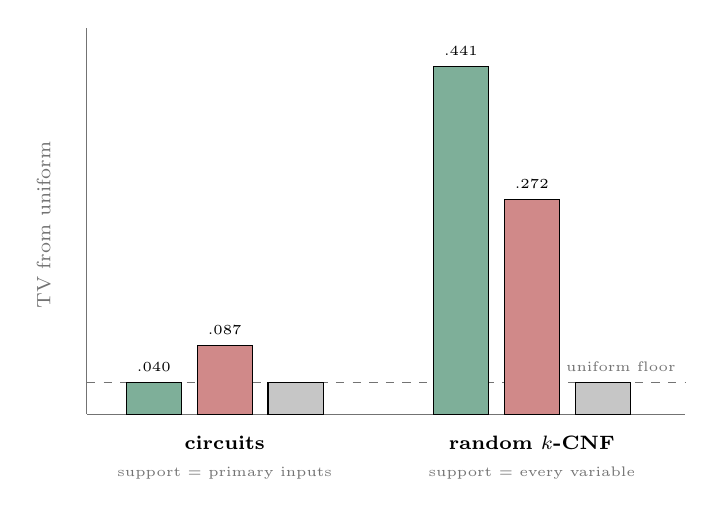
\begin{tikzpicture}[font=\scriptsize]
        \draw[gpapgray] (0,0) -- (7.6,0);
        \draw[gpapgray] (0,0) -- (0,4.9);
        \node[rotate=90,font=\scriptsize,gpapgray] at (-0.55,2.4) {TV from uniform};
        \draw[dashed,gpapgray] (0,0.4) -- (7.6,0.4);
        \node[font=\tiny,gpapgray,anchor=south east] at (7.6,0.42) {uniform floor};

        \draw[fill=gpapgreen!55] (0.5,0) rectangle (1.2,0.40);
        \draw[fill=gpapred!55]   (1.4,0) rectangle (2.1,0.87);
        \draw[fill=gray!45]      (2.3,0) rectangle (3.0,0.40);
        \node[font=\tiny,anchor=south] at (0.85,0.42) {.040};
        \node[font=\tiny,anchor=south] at (1.75,0.89) {.087};
        \node[font=\scriptsize,anchor=north] at (1.75,-0.15) {\textbf{circuits}};
        \node[font=\tiny,gpapgray,anchor=north] at (1.75,-0.55) {support $=$ primary inputs};

        \draw[fill=gpapgreen!55] (4.4,0) rectangle (5.1,4.41);
        \draw[fill=gpapred!55]   (5.3,0) rectangle (6.0,2.72);
        \draw[fill=gray!45]      (6.2,0) rectangle (6.9,0.40);
        \node[font=\tiny,anchor=south] at (4.75,4.43) {.441};
        \node[font=\tiny,anchor=south] at (5.65,2.74) {.272};
        \node[font=\scriptsize,anchor=north] at (5.65,-0.15) {\textbf{random $k$-CNF}};
        \node[font=\tiny,gpapgray,anchor=north] at (5.65,-0.55) {support $=$ every variable};
      \end{tikzpicture}}
      \\[0.3em]
      \rem{\good{green} $=$ \GPAP, \bad{red} $=$ CMSGen, grey $=$ exact-uniform control.}
    \end{column}
    \begin{column}{0.48\textwidth}
      \small
      \keyw{The instrument}: generate small formulas, enumerate their solutions exhaustively
      (solver-free), test $\chi^2$ $+$ TV against the \emph{known} uniform.
      \rem{Calibrated: 0/120 false positives on an exact-uniform control, 97\% power at TV 0.05.
      600 instances, 10{,}800 runs, \good{zero unsound rows}.}
      \\[0.5em]
      \good{On the flagship regime we are \emph{at} the floor} --- and CMSGen is not.
      \bad{On random $k$-CNF we are worse.} \keyw{Never quote the aggregate.}
      \\[0.5em]
      \keyw{An exactness knob}: at $B \ge |\text{support}|$ one round fixes the whole support and
      we discard failures --- exact rejection sampling, \good{24/24 at TV 0.0392}.
      \bad{Bounded by yield} when $p_{\text{accept}}$ is small.
    \end{column}
  \end{columns}
\end{frame}

% == 20 ================================================================
\begin{frame}{The uncomfortable one: our own bandit optimizes the wrong thing}
  \begin{center}
  \resizebox{0.86\textwidth}{!}{%
  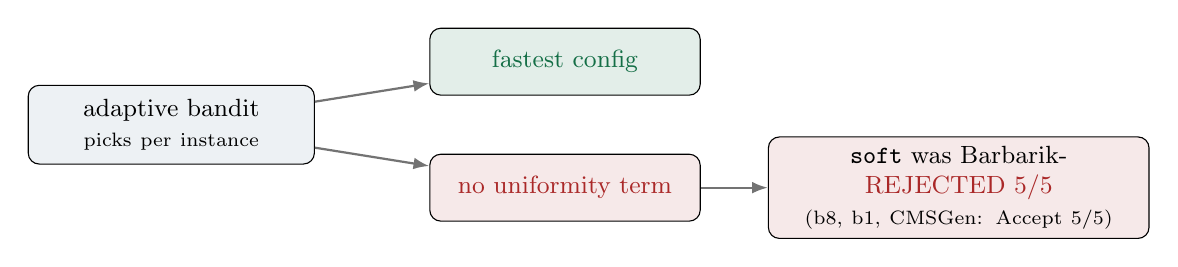
\begin{tikzpicture}[font=\small]
    \node[bx,text width=3.4cm,minimum height=1.0cm] (b) at (0,0) {adaptive bandit\\ \scriptsize picks per instance};
    \node[bxg,text width=3.2cm] (f) at (5.0,0.8) {\good{fastest config}};
    \node[bxr,text width=3.2cm] (u) at (5.0,-0.8) {\bad{no uniformity term}};
    \draw[ar] (b)--(f); \draw[ar] (b)--(u);
    \node[bxr,text width=4.6cm,font=\small] (s) at (10.0,-0.8)
      {\texttt{soft} was Barbarik-\bad{REJECTED 5/5}\\ \scriptsize (b8, b1, CMSGen: Accept 5/5)};
    \draw[ar] (u)--(s);
  \end{tikzpicture}}
  \end{center}
  \vspace{0.2em}
  \begin{columns}[T]
    \begin{column}{0.43\textwidth}
      \small
      \good{Acted on}: \texttt{soft} is opt-in behind \texttt{-{}-allow-soft}.
      \\[0.3em]
      \bad{\textbf{The price, on the published comparison}} --- the whole $357$-cell matrix run
      \emph{twice}, one flag changed: \bad{up to $4.6\times$ on deep sequential unrolls}
      ($14.0{\rightarrow}64.9\times$ at $T{=}50$), \good{${\approx}1.0\times$ on ISCAS-85,
      \texttt{sk\_} and HWMCC-random}.
    \end{column}
    \begin{column}{0.55\textwidth}
      \centering\scriptsize
      \begin{tabular}{@{}lrrr@{}}
        \toprule
        safe-arm success & cells & safe$/$soft & \texttt{soft} chosen \\
        \midrule
        $<10^{-4}$           & 13  & \bad{$0.119\times$}  & 5/13 \\
        $10^{-4}$--$10^{-2}$ & 22  & \bad{$0.313\times$}  & 12/22 \\
        $10^{-2}$--$0.5$     & 86  & $0.822\times$        & 24/86 \\
        $>0.5$               & 196 & \good{$0.988\times$} & 25/196 \\
        \bottomrule
      \end{tabular}
      \\[0.2em]
      \raggedright\small
      \good{\textbf{Nearly free where the sampler already works}}; expensive only where it does
      not --- exactly where \texttt{soft} wins.
    \end{column}
  \end{columns}
  \vspace{0.2em}
  \centering
  \rem{\keyw{The single geomean ($0.796\times$, headline $1.30\times$) pools regimes and is the
  least useful number.} Control: CMSGen $1.004\times$ between arms, $0/357$ cells differ in $M$ or
  $|\text{support}|$.}
\end{frame}

% == 21 ================================================================
\begin{frame}{Status, and what is open}
  \begin{columns}[T]
    \begin{column}{0.4\textwidth}
      \good{\textbf{Done}}
      \begin{itemize}\small
        \item engine: packed kernels, scalar $+$ WAVE, \texttt{libgpap}, three language faces
        \item sampler: pipeline, portfolios, mining, ELS, GPU projection
        \item front-ends: \texttt{.bench}, AIGER, ABC, simulation
        \item evaluation: resumable sweep, 3-seed medians, fair CMSGen, 3 GPU rivals
        \item uniformity: 3-tier readout, Barbarik, exact-oracle fuzzing
      \end{itemize}
    \end{column}
    \begin{column}{0.29\textwidth}
      \textbf{Open --- build}
      \begin{itemize}\small
        \item \keyw{uniformity-aware config choice} --- the one item that changes what a user gets
        \item per-instance encoder auto-pick
        \item state arena (${\sim}1.2\times$)
        \item ROCm port \rem{(no kernel work)}
        \item re-test the other applications
      \end{itemize}
    \end{column}
    \begin{column}{0.29\textwidth}
      \textbf{Open --- measure}
      \begin{itemize}\small
        \item \keyw{A100 rerun} --- every number is $K$-bound on a 12\,GB card
        \item multi-core CMSGen, QuickSampler
        \item break-even simulation throughput
        \item Barbarik $\times 10$ / ScalBarbarik
        \item one single-session ablation
      \end{itemize}
    \end{column}
  \end{columns}
\end{frame}

% == 22 ================================================================
\begin{frame}{Turning this into a paper}
  \begin{center}
  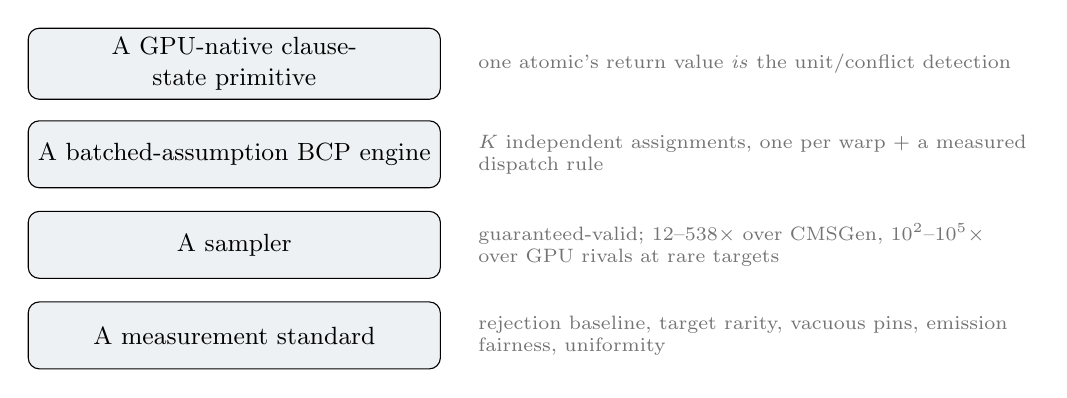
\begin{tikzpicture}[font=\small]
    \foreach \i/\txt/\sub in {
      0/{A GPU-native clause-state primitive}/{one atomic's return value \emph{is} the unit/conflict detection},
      1/{A batched-assumption BCP engine}/{$K$ independent assignments, one per warp $+$ a measured dispatch rule},
      2/{A sampler}/{guaranteed-valid; $12$--$538\times$ over CMSGen, $10^2$--$10^5\times$ over GPU rivals at rare targets},
      3/{A measurement standard}/{rejection baseline, target rarity, vacuous pins, emission fairness, uniformity}} {
      \node[bx,text width=5.0cm,anchor=west] at (0,-\i*1.15) {\txt};
      \node[anchor=west,font=\scriptsize,gpapgray,text width=7.0cm] at (5.6,-\i*1.15) {\sub};
    }
  \end{tikzpicture}
  \end{center}
  \vspace{0.6em}
  \centering
  \small
  \good{Have}: every figure on these slides, the 357-row sweep, three rival tables, the uniformity
  campaign.\\
  \bad{Need}: the A100 column, a multi-core CMSGen row, one single-session ablation, and a
  decision on the bandit/uniformity trade.
\end{frame}

% == 23 ================================================================
\appendix

% Frames moved out of the main line 2026-08-06 (engine feature list; the 4080-laptop headline).
% ---------------------------------------------------------------------------
%  GPAP — BACKUP slides. A deck of its own: detail an advisor may ask about,
%  deliberately kept out of the talk so the main narrative runs engine ->
%  application -> evidence without interruption.
%
%  Compile:  pdflatex backup_slides.tex   (twice)
%  Shares gpap_style.tex with the main deck, so colours and macros cannot drift.
% ---------------------------------------------------------------------------
% ---------------------------------------------------------------------------
%  Shared preamble for the GPAP decks (gpap_overview.tex and backup_slides.tex).
%  Kept in one file so the two never drift apart in colour, macros or theme.
%  Deps: base beamer + booktabs + tikz. Nothing exotic; compiles on Overleaf.
% ---------------------------------------------------------------------------
\documentclass[aspectratio=169,11pt]{beamer}

\usetheme{Boadilla}
\usecolortheme{whale}
\setbeamertemplate{navigation symbols}{}
\setbeamerfont{frametitle}{size=\large}
\setbeamertemplate{itemize items}[circle]

\usepackage[T1]{fontenc}
\usepackage[utf8]{inputenc}
\usepackage{amsmath,amssymb}
\usepackage{booktabs}
\usepackage{xcolor}
\usepackage{tikz}
\usetikzlibrary{positioning,arrows.meta}

\definecolor{gpapblue}{RGB}{31,78,121}
\definecolor{gpapred}{RGB}{170,40,40}
\definecolor{gpapgreen}{RGB}{20,110,70}
\definecolor{gpapgray}{RGB}{115,115,115}
\definecolor{gpapamber}{RGB}{180,120,20}

\newcommand{\good}[1]{\textcolor{gpapgreen}{#1}}
\newcommand{\bad}[1]{\textcolor{gpapred}{#1}}
\newcommand{\rem}[1]{{\footnotesize\textcolor{gpapgray}{#1}}}
\newcommand{\NC}{\textsc{NobleCount}}
\newcommand{\GPAP}{\textsc{Gpap}}
\newcommand{\keyw}[1]{\textcolor{gpapblue}{\textbf{#1}}}

\tikzset{
  bx/.style  = {draw, rounded corners, align=center, minimum height=0.85cm, fill=gpapblue!8,  font=\small},
  bxg/.style = {draw, rounded corners, align=center, minimum height=0.85cm, fill=gpapgreen!12, font=\small},
  bxr/.style = {draw, rounded corners, align=center, minimum height=0.85cm, fill=gpapred!10,  font=\small},
  bxn/.style = {draw, rounded corners, align=center, minimum height=0.85cm, fill=black!4,     font=\small},
  ar/.style  = {-{Latex[length=2mm]}, thick, gpapgray},
}



\title[GPAP backup]{\GPAP{} --- backup slides}
\subtitle{detail behind the main deck}
\author[Y. Shalmon]{Yogev Shalmon}
\institute[Technion]{Technion --- Faculty of Data and Decision Sciences}
\date{\today}

\begin{document}

\begin{frame}[plain]
  \titlepage
\end{frame}

% --- was frame 8: the engine feature list (too technical for the main line) ---
\begin{frame}{Backup: the engine, in features}
  \begin{columns}[T]
    \begin{column}{0.48\textwidth}
      \begin{itemize}\small
        \item one packed \texttt{int32} per clause --- update is a single atomic
        \item assignment as a bitmap --- one atomic gives dedup \emph{and} contradiction
        \item two propagate kernels, \keyw{auto-dispatched} per formula
        \item the whole decide$+$propagate trajectory \keyw{fused into one launch}
      \end{itemize}
    \end{column}
    \begin{column}{0.48\textwidth}
      \begin{itemize}\small
        \item $K$ sized analytically from free VRAM; unit-flush cached at construction
        \item readout stays \keyw{on device} --- only counts and projections cross the bus
        \item two packed splits chosen per formula; out-of-envelope formulas rejected, never
          silently degraded
      \end{itemize}
    \end{column}
  \end{columns}
  \vspace{0.6em}
  \begin{block}{Bottom line}
    \centering
    \good{\textbf{Up to $5.7\times$ end-to-end}} over the pre-WAVE engine --- with
    \keyw{bit-identical model sets} at every step.
  \end{block}
  \rem{Negative results, kept because they cost weeks: classic \textbf{2-watched-literals on GPU
  is $1.8$--$2.6\times$ slower} than \NC-style counting, on ${\sim}5\times$ the per-row state;
  1-byte clause state, clause renumbering and multi-warp tiles all measured out.}
\end{frame}

% --- was frame 13/14: the 4080-laptop column, and the CPU-dependence analysis ---
\begin{frame}{Backup: the same suite on two machines --- and why the ratio moved}
  \centering
  \small
  \begin{tabular}{@{}llrrr@{}}
    \toprule
    family & targets & 4080 laptop & \textbf{Colab L4} & wins (L4) \\
    \midrule
    ITC'99 $+$ ISCAS-89 seq, $T{=}25$ & \keyw{rare} & $36.5\times$ & $39.1\times$ & 17/18 \\
    ISCAS-85 combinational            & \keyw{rare} & $538\times$  & $615\times$  & 10/10 \\
    HWMCC'17, $T{=}25$                & \keyw{rare} & $156\times$  & $196\times$  & 7/7 \\
    EPFL combinational                & \keyw{rare} & $6.4\times$  & $9.4\times$  & 13/17 \\
    Sketch / \texttt{sk\_} CNFs       & ---         & $46.2\times$ & $98.9\times$ & 27/29 \\
    \bottomrule
  \end{tabular}
  \\[1.0em]
  \begin{columns}[T]
    \begin{column}{0.48\textwidth}
      \bad{\textbf{Every ratio is higher on the L4 --- and none of it is \GPAP{}.}}
      \\[0.3em]
      \small
      Paired on identical cells: \GPAP{} $0.96\times$ (same engine, slightly slower card) while
      \keyw{CMSGen runs at $0.41\times$} --- a Xeon @ 2.2\,GHz against an \texttt{i7-13800H}.
      \rem{CMSGen's own propagation \emph{and} decision counters independently both give
      $0.413\times$.}
    \end{column}
    \begin{column}{0.48\textwidth}
      \good{\textbf{Hence the rule: never quote a ratio without the CPU.}}
      \\[0.3em]
      \small
      CMSGen is single-core, so the number is as much a property of the host as of the sampler.
      Otherwise a reviewer reads $98.9\times$ and correctly calls it a rigged baseline.
      \rem{The same caution applies in advance to the Technion cluster runs.}
    \end{column}
  \end{columns}
\end{frame}

% --- the two reporting corrections, kept for the record ---
\begin{frame}{Backup: two corrections we made to our own headline}
  \begin{block}{One rule}
    \centering
    \keyw{A cell that measures the \emph{instance} instead of the \emph{sampler} does not belong
    in a geomean.}
  \end{block}
  \vspace{0.4em}
  \small
  \textbf{(i) Vacuous output pins.} \texttt{b02/b05/b07/s526} have constant outputs at $T{=}25$, so
  pinning them is a tautology and \emph{any} sampler scores ${\sim}100\%$. Including them read
  \bad{$47.7\times$} on the sequential-rare column instead of \good{$36.5\times$} --- an inflation
  of up to $1.9\times$, falling almost entirely on the column we tell people to quote.
  \\[0.6em]
  \textbf{(ii) Instances that need no search at all.} A few cells emit samples with \keyw{zero
  decisions and zero implications}: after propagation the support is unconstrained, so ``sampling''
  is a random-bit readout at $240$M/s. Worse, picking the best encoder per instance
  \emph{prefers} them, because they carry the family's highest ratio. Including them read EPFL
  \bad{$12.7\times$} instead of \good{$6.4\times$}, and \texttt{sk\_} \bad{$48.5\times$} instead of
  \good{$46.2\times$}.
  \\[0.6em]
  \rem{Both are now enforced in the table generator and re-checked by a verifier, so they cannot
  come back. The same generator produces the paper tables and these slides.}
\end{frame}

% --- was the main-deck status frame; the roadmap detail belongs off the main line ---
\begin{frame}{Backup: status, and what is open}
  \begin{columns}[T]
    \begin{column}{0.4\textwidth}
      \good{\textbf{Done}}
      \begin{itemize}\small
        \item engine: packed kernels, scalar $+$ WAVE, \texttt{libgpap}, three language faces
        \item sampler: pipeline, portfolios, mining, ELS, GPU projection
        \item front-ends: \texttt{.bench}, AIGER, ABC, simulation
        \item evaluation: resumable sweep, 3-seed medians, fair CMSGen, 3 GPU rivals
        \item uniformity: 3-tier readout, Barbarik, exact-oracle fuzzing
      \end{itemize}
    \end{column}
    \begin{column}{0.29\textwidth}
      \textbf{Open --- build}
      \begin{itemize}\small
        \item \keyw{uniformity-aware config choice} --- the one item that changes what a user gets
        \item per-instance encoder auto-pick
        \item state arena (${\sim}1.2\times$)
        \item ROCm port \rem{(no kernel work)}
        \item re-test the other applications
      \end{itemize}
    \end{column}
    \begin{column}{0.29\textwidth}
      \textbf{Open --- measure}
      \begin{itemize}\small
        \item \keyw{A100 rerun} --- every number is $K$-bound on a 12\,GB card
        \item multi-core CMSGen, QuickSampler
        \item break-even simulation throughput
        \item Barbarik $\times 10$ / ScalBarbarik
        \item one single-session ablation
      \end{itemize}
    \end{column}
  \end{columns}
\end{frame}

% --- was a main-deck frame: the cross-GPU rival check ---
\begin{frame}{Backup: does the rival verdict survive a different GPU?}
  \centering
  \small
  \begin{tabular}{@{}llrrc@{}}
    \toprule
    rival & protocol & \multicolumn{2}{c}{GPAP $/$ rival (geomean)} & GPAP wins \\
    \cmidrule(lr){3-4}
     & & 4080 laptop & \textbf{L4} & on L4 \\
    \midrule
    DEMOTIC   & their ISCAS-85 pins     & $2.9\times$     & $2.5\times$     & \good{19/20} \\
    DEMOTIC   & our \keyw{rare} pins    & $7{,}704\times$ & $2{,}427\times$ & \good{16/16} \\
    Recurrent & our \keyw{rare} pins    & $599\times$     & $422\times$     & \good{3/3} \\
    HTS       & our CNFs, both encoders & ---             & $2{,}042\times$ & \good{10/10} \\
    \bottomrule
  \end{tabular}
  \\[1.0em]
  \begin{columns}[T]
    \begin{column}{0.48\textwidth}
      \good{\textbf{What transfers: the verdict.}}
      \\[0.3em]
      Win counts are \emph{identical} on both cards.
    \end{column}
    \begin{column}{0.48\textwidth}
      \bad{\textbf{What does not: the magnitude.}}
      \\[0.3em]
      \keyw{Read these as orders of magnitude.}
    \end{column}
  \end{columns}
  \vspace{0.5em}
  \centering
  \rem{At rare pins the rival scores ${\approx}0$, so the ratio has a near-zero denominator.
  \bad{Honest}: \texttt{c1355} loses on both cards.}
\end{frame}

\begin{frame}{Backup: numbers on hand}
  \footnotesize
  \begin{columns}[T]
    \begin{column}{0.48\textwidth}
      \textbf{Engine}
      \begin{itemize}
        \item vs pre-WAVE: b14 $5.7\times$, b12 $2.8\times$, b04 $1.8\times$, b03 $1.5\times$
        \item rates: b03 631k, b06 945k, b04 81k, b12 50k, b14 4.0k attempts/s
        \item C++ port: $1.013\times$ geomean, identical model sets
        \item portability: 75/1273 CUDA lines, 18 driver calls, 29/29 specializations cross-compile
      \end{itemize}
      \textbf{Encoder}
      \begin{itemize}
        \item ABC shrink $2.2$--$7.8\times$ clauses; at rare targets bimodal (unlocks b14, collapses b13)
        \item \texttt{fast} vs \texttt{full}: b15 encode $99$\,s $\rightarrow$ ${\le}4$\,s
      \end{itemize}
    \end{column}
    \begin{column}{0.48\textwidth}
      \textbf{Uniformity}
      \begin{itemize}
        \item 600 instances, 10{,}800 runs, 0 unsound; controls 0/600 FP, 600/600 power
        \item $B\ge|\text{sup}|$: 24/24 ok, TV 0.0392 (theory floor 0.0399)
        \item circuits 0.040 vs CMSGen 0.087; CNF 0.441 vs 0.272
        \item \texttt{soft}: Reject 5/5 in 156--936 samples, TV median 0.694
      \end{itemize}
      \textbf{Baselines / method}
      \begin{itemize}
        \item CMSGen emission $= 5.3\times$ its wall (373\,MB on 27.sk)
        \item rare-target amplification $500$--$500{,}000\times$
        \item SM clock 615--1710\,MHz while $>$90\% busy; draw noise $\pm40\%$
      \end{itemize}
    \end{column}
  \end{columns}
\end{frame}

\end{document}


\begin{frame}{Backup: numbers on hand}
  \footnotesize
  \begin{columns}[T]
    \begin{column}{0.48\textwidth}
      \textbf{Engine}
      \begin{itemize}
        \item vs pre-WAVE: b14 $5.7\times$, b12 $2.8\times$, b04 $1.8\times$, b03 $1.5\times$
        \item rates: b03 631k, b06 945k, b04 81k, b12 50k, b14 4.0k attempts/s
        \item C++ port: $1.013\times$ geomean, identical model sets
        \item portability: 75/1273 CUDA lines, 18 driver calls, 29/29 specializations cross-compile
      \end{itemize}
      \textbf{Encoder}
      \begin{itemize}
        \item ABC shrink $2.2$--$7.8\times$ clauses; at rare targets bimodal (unlocks b14, collapses b13)
        \item \texttt{fast} vs \texttt{full}: b15 encode $99$\,s $\rightarrow$ ${\le}4$\,s
      \end{itemize}
    \end{column}
    \begin{column}{0.48\textwidth}
      \textbf{Uniformity}
      \begin{itemize}
        \item 600 instances, 10{,}800 runs, 0 unsound; controls 0/600 FP, 600/600 power
        \item $B\ge|\text{sup}|$: 24/24 ok, TV 0.0392 (theory floor 0.0399)
        \item circuits 0.040 vs CMSGen 0.087; CNF 0.441 vs 0.272
        \item \texttt{soft}: Reject 5/5 in 156--936 samples, TV median 0.694
      \end{itemize}
      \textbf{Baselines / method}
      \begin{itemize}
        \item CMSGen emission $= 5.3\times$ its wall (373\,MB on 27.sk)
        \item rare-target amplification $500$--$500{,}000\times$
        \item SM clock 615--1710\,MHz while $>$90\% busy; draw noise $\pm40\%$
      \end{itemize}
    \end{column}
  \end{columns}
\end{frame}

% Full L4 result tables — GENERATED from the experiment JSONs by eval/slide_tables.py, so no
% number on these frames is ever transcribed by hand. Regenerate with:
%   eval/slide_tables.py --cmsgen .experiments/cmsgen_l4_2026-08-03 \
%       --rivals .experiments/l4_rivals --out docs/slides/l4_results.tex
% GENERATED by eval/slide_tables.py — do not edit by hand.
% source: .experiments/cmsgen_l4_2026-08-03 + .experiments/l4_rivals

\begin{frame}{Appendix: every CMSGen family measured on the L4}
  \centering \scriptsize
  \begin{tabular}{@{}llrrrrr@{}}
    \toprule
    family & targets & inst & GPAP$/$CMSGen & \textbf{no-vac} & wins & CMSGen 0 \\
    \midrule
    ITC'99 $+$ ISCAS-89 seq, $T{=}25$ & \keyw{rare} & 19 & $58.2$$\times$ & $39.1$$\times$ & 17/18 & 1 \\
    ITC'99 $+$ ISCAS-89 seq, $T{=}50$ & \keyw{rare} & 19 & $26.3$$\times$ & $14.0$$\times$ & 15/16 & 3 \\
    ITC'99 $+$ ISCAS-89 seq, $T{=}25$ & random & 19 & $191.4$$\times$ & $183.3$$\times$ & 18/18 & 1 \\
    ITC'99 $+$ ISCAS-89 seq, $T{=}50$ & random & 19 & $164.6$$\times$ & $147.0$$\times$ & 19/19 & 7 \\
    ISCAS-85 combinational & \keyw{rare} & 10 & $615.4$$\times$ & --- & 10/10 & 1 \\
    ISCAS-85 combinational & random & 10 & $636.1$$\times$ & --- & 10/10 & 1 \\
    HWMCC'17, $T{=}25$ & \keyw{rare} & 7 & $195.6$$\times$ & --- & 7/7 & 5 \\
    HWMCC'17, $T{=}50$ & \keyw{rare} & 7 & $421.5$$\times$ & --- & 7/7 & 6 \\
    HWMCC'17, $T{=}25$ & random & 7 & $263.8$$\times$ & --- & 7/7 & 5 \\
    HWMCC'17, $T{=}50$ & random & 7 & $520.6$$\times$ & --- & 7/7 & 6 \\
    EPFL combinational & \keyw{rare} & 20 & $29.0$$\times$ & --- & 13/16 & 1 \\
    EPFL combinational & random & 20 & $19.5$$\times$ & --- & 12/16 & 1 \\
    Sketch / \texttt{sk\_} projected CNFs & --- & 29 & $113.1$$\times$ & --- & 27/28 & 0 \\
    \bottomrule
  \end{tabular}
  \\[0.7em]
  \rem{\textbf{357 cells, 193 instance-slots, 0 skipped, 0 errors}. GPU \textbf{NVIDIA L4}, CPU \textbf{Intel(R) Xeon(R) CPU @ 2.20GHz}.
  \keyw{no-vac} drops \texttt{b02/b05/b07/s526}, whose outputs are constant at $T{=}25$ so  any sampler scores ${\sim}100\%$ --- quote it, not the raw column.
  \keyw{CMSGen 0} counts instances where CMSGen emitted \emph{zero} samples in budget:  outright wins, but ratio $=\infty$, so they are EXCLUDED from every geomean above.  The numbers are therefore conservative.
}
\end{frame}

\begin{frame}{Appendix: every GPU rival measured on the L4}
  \centering \scriptsize
  \begin{tabular}{@{}llrrrr@{}}
    \toprule
    rival & protocol & cells & GPAP$/$rival & wins & rival failed \\
    \midrule
    DEMOTIC & their ISCAS-85 pins & 20 & $2.5$$\times$ & 19/20 & 0 \\
    DEMOTIC & our \keyw{rare} pins & 18 & $2,426.6$$\times$ & 16/16 & 0 \\
    Recurrent & their target table & 9 & $4.4$$\times$ & 6/6 & 3 \\
    Recurrent & our \keyw{rare} pins & 9 & $634.9$$\times$ & 4/5 & 3 \\
    HTS & our CNFs (both encoders) & 18 & $1,584.4$$\times$ & 11/12 & 3 \\
    \bottomrule
  \end{tabular}
  \\[0.7em]
  \rem{Their metric: unique solutions $/$ their \texttt{model\_runtime}, which excludes  their model build while ours includes construction. \keyw{rival failed} = timeout or  no gradient path; those rows are reported, never folded in as a zero. Rows where the  rival scored $0$ are excluded from the geomean for the same reason as above.}
\end{frame}

\begin{frame}{Appendix: uniformity against an exact oracle}
  \centering \scriptsize
  \begin{tabular}{@{}lrrrr@{}}
    \toprule
    sampler & \multicolumn{2}{c}{circuit} & \multicolumn{2}{c}{random $k$-CNF} \\
    \cmidrule(lr){2-3}\cmidrule(lr){4-5}
     & median TV & skewed & median TV & skewed \\
    \midrule
    \rem{\texttt{ctl:uniform}} & $0.0395$ & 0/36 & $0.0401$ & 0/36 \\
    \rem{\texttt{ctl:tv0.05}} & $0.0577$ & 36/36 & $0.0580$ & 36/36 \\
    \texttt{gpap:b1} & $0.1109$ & 18/36 & $0.4368$ & 36/36 \\
    \texttt{gpap:b8} & $0.0401$ & 10/36 & $0.4033$ & 36/36 \\
    \bad{\texttt{gpap:soft}} & $0.6255$ & 24/36 & $0.7605$ & 36/36 \\
    \texttt{gpap:b32} & $0.0399$ & 0/36 & $0.0401$ & 0/36 \\
    \texttt{gpap:b64} & $0.0399$ & 0/36 & $0.0401$ & 0/36 \\
    \texttt{cmsgen} & $0.0945$ & 25/36 & $0.2576$ & 36/36 \\
    \bottomrule
  \end{tabular}
  \\[0.7em]
  \rem{72 generated instances whose ENTIRE solution set is enumerated by brute force, so the target is known exactly; $\chi^2$ over 3 seeds, Fisher-combined, $\alpha=0.001$. \good{0 unsound emissions}. \keyw{The controls calibrate the instrument}: \texttt{ctl:uniform} is exactly uniform and must NOT be flagged; \texttt{ctl:tv0.05} is skewed by a known amount and must be. \bad{\texttt{soft} is why it is opt-in} --- and $B\ge|\text{support}|$ (\texttt{b32}/\texttt{b64}) is exactly uniform, because discarding conflicts IS rejection sampling.}
\end{frame}



\end{document}
